\documentclass[margin=0px]{article}

\usepackage{listings}
\usepackage[utf8]{inputenc}
\usepackage{graphicx}
\usepackage{float}
\usepackage[a4paper, margin=0.7in]{geometry}
\usepackage{amsthm}
\usepackage{amssymb}
\usepackage{fancyhdr}
\usepackage{setspace}

\onehalfspacing

\makeatletter
\renewcommand\paragraph{%
	\@startsection{paragraph}{4}{0mm}%
	{-\baselineskip}%
	{.5\baselineskip}%
	{\normalfont\normalsize\bfseries}}
\makeatother

\renewcommand{\figurename}{ábra}

\newenvironment{tetel}[1]{\paragraph{#1 \\}}{}

\pagestyle{fancy}
\lhead{\it{PTI BSc Záróvizsga tételek}}
\rhead{13.1 Logika}

\title{\textbf{{\Large ELTE IK - Programtervező Informatikus BSc} \vspace{0.2cm} \\ {\huge Záróvizsga tételek}} \vspace{0.3cm} \\ 13.1 Logika}
\author{}
\date{}

\begin{document}
\maketitle

\begin{tetel}{Logika}
    Ítéletkalkulus és elsőrendű predikátumkalkulus: szintaxis, szemantika, ekvivalens átalakítások, a szemantikus következmény fogalma, rezolúció.
\end{tetel}

\section{Logika}

\subsection{Alapfogalmak}

A logika tárgya az emberi gondolkodási folyamat vizsgálata és
helyes gondolkodási formák keresése, illetve létrehozása.\\

\noindent Fogalmak:
\begin{enumerate}
    \item	\textbf{Állítás}: Olyan kijelentés, melynek logikai értéke (igaz
          volta) eldönthető, tetszőleges kontextusban igaz vagy hamis. Azt mondjuk,
          hogy egy állítás igaz, ha információtartalma megfelel a valóságnak (a tényeknek),
          és hamis az ellenkező esetben.

          A mindennapi beszédben használt kijelentő mondatok legtöbbször nem állítások, mivel
          a mondat tartalmába a kontextus is beleszámít: időpont, környezet állapota, általános műveltség
          bizonyos szintje, stb. (pl. nem állítás az, hogy "ma reggel 8-kor sütött a nap", de állítás pl. az, hogy
          "minden páros szám osztható 2-vel").

    \item	\textbf{Igazságérték}: Az igazságértékek halmaza $\mathbb{L}=\left\{igaz,hamis\right\}$.

    \item	\textbf{Gondolkodási forma}: Gondolkodási forma alatt egy olyan $(F,A)$ párt értünk, ahol
          $A$ állítás, $F=\left\{A_{1},A_{2},...,A_{n}\right\}$ pedig állítások egy halmaza.

          A gondolkodásforma helyes, ha minden esetben, amikor $F$ minden állítása
          igaz, akkor $A$ is igaz.
\end{enumerate}

\subsection{Ítéletkalkulus}

\subsubsection{Az ítéletlogika szintaxisa}

\paragraph{Az ítéletlogika ábécéje}
Az ítéletlogika ábécéje $V_{0}=V_{v} \cup \left\{(,)\right\} \cup \left\{\neg, \wedge, \vee, \supset\right\}$, ahol $V_{v}$ az
ítéletváltozók halmaza. Tehát $V_{0}$ az ítéletváltozókat, a zárójeleket, és a logikai műveletek jeleit tartalmazza.

\paragraph{Az ítéletlogika nyelve}
Az ítéletlogika nyelve ($\mathcal{L}_{0}$) ítéletlogikai formulákból áll, amelyek a következőképpen állnak elő:
\begin{enumerate}
    \item	Minden ítéletváltozó ítéletlogikai formula. Ezek az úgynevezett prímformulák (vagy atomi formulák).

    \item	Ha $A$ ítéletlogikai formula, akkor $\neg A$ is az.

    \item	Ha $A$ és $B$ ítéletlogikai formulák, akkor $(A \wedge B)$, $(A \vee B)$ és $(A \supset B)$ is
          ítéletlogikai formulák.

    \item	Minden ítéletlogikai formula az 1-3. szabályok véges sokszori alkalmazásával áll elő.
\end{enumerate}

\noindent \textbf{Literál}: Ha $X$ ítéletváltozó, akkor az $X$ és $\neg X$ formulák literálok, amelyek alapja $X$.\\

\noindent \textbf{Közvetlen részformula}:
\begin{enumerate}
    \item	Prímformulának nincs közvetlen részformulája.

    \item	$\neg A$ közvetlen részformulája $A$.

    \item	$A \circ B$ ($\circ$ a $\wedge, \vee, \supset$ binér összekötőjelek egyike) közvetlen részformulái $A$ (bal oldali)
          és $B$ (jobb oldali).
\end{enumerate}

\noindent \textbf{Részformula}: Legyen $A \in \mathcal{L}_{0}$ egy ítéletlogikai formula. Ekkor $A$ részformuláinak
halmaza a legszűkebb olyan halmaz, melynek
\begin{enumerate}
    \item	eleme az $A$, és

    \item	ha a C formula eleme, akkor C közvetlen részformulái is elemei.

\end{enumerate}

\noindent \textbf{Szerkezeti fa}: Egy C formula szerkezeti fája egy olyan véges rendezett fa, melynek csúcsai formulák,
\begin{enumerate}
    \item	gyökere C,

    \item	a $\neg A$ csúcsának pontosan egy gyermeke van, az $A$,

    \item	a $A \circ B$ csúcsának pontosan két gyermeke van, rendre az $A$ és $B$ formulák,

    \item	levelei prímformulák.
\end{enumerate}

\begin{figure}[H]
    \centering
    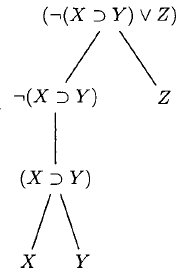
\includegraphics[width=0.3\linewidth]{img/szerkfa}
    \caption{Példa szerkezeti fára.}
    \label{fig:szerkfa}
\end{figure}

\noindent \textbf{Logikai összetettség}: Egy formula logikai összetettsége a benne található logikai összekötőjelek száma.\\

\noindent \textbf{Művelet hatásköre}: Egy művelet hatásköre a formula részformulái közül az
a legkisebb logikai összetettségű részformula, melyben az adott művelet előfordul.\\

\noindent \textbf{Fő logikai összekötőjel}: Egy formula fő logikai összekötőjele az az összekötőjel, amelynek
hatásköre maga a formula.\\

\noindent \textbf{Precedencia}: A logikai összekötőjelek precedenciája csökkenő sorrendben a következő: $\neg, \wedge, \vee, \supset$.\\

A definíciók alapján egyértelmű, hogy egy \textit{teljesen zárójelezett formulában} mi a logikai összekötőjelek hatásköre és mi a fő
logikai összekötőjel. Most megmutatjuk, hogy egy formulában milyen esetekben és mely részformulákat határoló zárójelek hagyhatóak el úgy, hogy a logikai összekötőjelek hatásköre ne változzon. A részformulák közül a prímformuláknak és a negációs formuláknak nincs külső zárójelpárja, ezért csak az $(A \circ B)$ alakú részformulákról kell eldöntenünk, hogy írható-e helyettük $A \circ B$. A zárójelek elhagyását
mindig a formula külső zárójelpárjának (ha van ilyen) elhagyásával kezdjük. Majd ha egy részformulában már megvizsgáltuk a külső zárójelelhagyás kérdését, utána ezen részformula közvetlen részformuláinak külső zárójeleivel foglalkozunk. Két eset lehetséges:

\begin{enumerate}
    \item	A részformula egy negációs formula, melyben az $(A \circ B)$ alakú közvetlen részformula külső zárójelei nem hagyhatók el.

    \item	A részformula egy $(A \bullet B)$ vagy $A \bullet B$ alakú formula, melynek $A$ és $B$ közvetlen részformuláiban kell dönteni a külső zárójelek sorsáról. Ha az $A$ formula $A_{1} \circ A_{2}$ alakú, akkor $A$ külső zárójelpárja akkor hagyható el, ha $\circ$ nagyobb precedenciájú, mint $\bullet$. Ha a $B$ formula $B_{1} \circ B_{2}$ alakú, akkor $B$ külső zárójelpárja akkor hagyható el, ha $\circ$ nagyobb vagy egyenlő precedenciájú, mint $\bullet$.

    \item	Ha egy $(A \wedge B)$ vagy $A \wedge B$ alakú formula valamely közvetlen részformulája szintén konjunkció, illetve egy
          $(A \vee B)$ vagy $A \vee B$ alakú formula valamely közvetlen részformulája szintén diszjunkció, akkor az ilyen részformulákból a külső zárójelpár elhagyható.
\end{enumerate}

\noindent \textbf{Formulaláncok}: A zárójelek elhagyására vonatkozó megállapodásokat figyelembe véve úgynevezett konjunkciós, diszjunkciós, illetve implikációs formulaláncokat is nyerhetünk. Ezek alakja $A_{1} \wedge ... \wedge A_{n}$, $A_{1} \vee ... \vee A_{n}$, illetve
$A_{1} \supset ... \supset A_{n}$ Ezeknek a láncformuláknak a fő logikai összekötőjelét a következő zárójelezési megállapodással fogjuk meghatározni: $(A_{1} \wedge (A_{2} \wedge ... \wedge (A_{n-1} \wedge A_{n})...))$, $(A_{1} \vee (A_{2} \vee ... \vee (A_{n-1} \vee A_{n})...))$, illetve $(A_{1} \supset (A_{2} \supset ... \supset (A_{n-1} \supset A_{n})...))$

\subsubsection{Az ítéletlogika szemantikája}

\noindent \textbf{Interpretáció}: $\mathcal{L}_{0}$ interpretációján egy $\mathcal{I} : V_{v} \to \mathbb{L}$ függvényt értünk, mely minden ítéletváltozóhoz egyértelműen hozzárendel egy igazságértéket.\\

\noindent \textbf{Boole-értékelés}: $\mathcal{L}_{0}$-beli formulák $\mathcal{I}$ \textit{interpretációbeli Boole-értékelése} a következő $\mathcal{B}_{\mathcal{I}} : \mathcal{L}_{0} \to \mathbb{L}$ függvény:

\begin{enumerate}
    \item ha $A$ prímformula, akkor $\mathcal{B}_{\mathcal{I}}(A) = \mathcal{I}(A)$,

    \item $\mathcal{B}_{\mathcal{I}}(\neg A)$ legyen $\neg \mathcal{B}_{\mathcal{I}}(A) $,

    \item $\mathcal{B}_{\mathcal{I}}(A \wedge B)$ legyen $\mathcal{B}_{\mathcal{I}}(A) \wedge \mathcal{B}_{\mathcal{I}}(B)$,

    \item $\mathcal{B}_{\mathcal{I}}(A \vee B)$ legyen $\mathcal{B}_{\mathcal{I}}(A) \vee \mathcal{B}_{\mathcal{I}}(B)$,

    \item $\mathcal{B}_{\mathcal{I}}(A \supset B)$ legyen $\mathcal{B}_{\mathcal{I}}(A) \supset \mathcal{B}_{\mathcal{I}}(B)$,
\end{enumerate}

\noindent \textbf{Bázis}: A formula ítéletváltozóinak egy rögzített sorrendje.\\

\noindent \textbf{Szemantikus fa}: Egy formula különböző interpretációit szemantikus fa segítségével szemléltethetjük. A szemantikus
fa egy olyan bináris fa, amelynek $i$. szintje ($i>=1$) a bázis $i$. ítéletváltozójához tartozik, és minden csúcsából két él indul, az
egyik a szinthez rendelt ítéletváltozóval, a másik annak negáltjával címkézve. Az $X$ ítéletváltozó esetén az $X$ címke jelentse azt, hogy az $X$ \textit{igaz} az adott interpretációban, a $\neg X$ címke pedig azt, hogy \textit{hamis} az adott interpretációban. A szemantikus fa
minden ága egy-egy lehetséges interpretációt reprezentál. Egy $n$ változós formula esetén minden ág $n$ hosszú, és a fának $2^{n}$ ága van és az összes lehetséges interpretációt tartalmazza.

\begin{figure}[H]
    \centering
    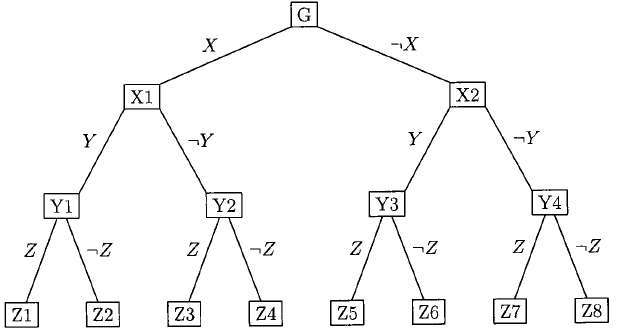
\includegraphics[width=0.6\linewidth]{img/szemantikusfa}
    \caption{Az X,Y,Z ítéletváltozókat tartalmazó formula szemantikus fája.}
    \label{fig:szemantikusfa}
\end{figure}

\noindent \textbf{Igazságtábla}: Egy $n$ változós formula igazságtáblája egy $n+1$ oszlopból és $2^{n}$ sorból álló táblázat.
A táblázat fejlécében az $i$. oszlophoz ($1<=i<=n$) a formula bázisának $i$. ítéletváltozója, az $n+1$. oszlophoz maga a formula
van hozzárendelve. Az első $n$ oszlopban az egyes sorokhoz megadjuk rendre a formula különböző interpretációit, majd a formula
oszlopába minden sorba beírjuk a formula - a sorhoz tartozó interpretációbeli Boole-értékeléssel kapott - igazságértékét.\\

\noindent \textbf{A logikai műveletek igazságtáblája}:

\begin{table}[H]
    \begin{tabular}{ll|lllll}
        X & Y & $\neg X$ & $X \wedge Y$ & $X \vee Y$ & $ X \supset Y$ & \\ \hline
        i & i & h        & i            & i          & i              & \\
        i & h & h        & h            & i          & h              & \\
        h & i & i        & h            & i          & i              & \\
        h & h & i        & h            & h          & i              &
    \end{tabular}
\end{table}

\noindent \textbf{Igazhalmaz, hamishalmaz}: Egy $A$ formula igazhalmaza $(A^{i})$
azon interpretációk halmaza, melyen a formula igazságértékelése igaz. Az $A$ formula
hamishalmaza $(A^{h})$ pedig azon interpretációk halmaza, melyekre a formula igazságértékelése hamis.\\

\noindent \textbf{Igazságértékelés függvény}:  Olyan függvény, amely minden formulához hozzárendeli az igazhalmazát ($\varphi A^{i}$) vagy
a hamishalmazát ($\varphi A^{h}$).\\

Legyen $A$ egy tetszőleges ítéletlogikai formula. Határozzuk meg $A$-hoz az interpretációira vonatkozó $\varphi A^{i}$, illetve
$\varphi A^{h}$ feltételeket a következőképpen:

\begin{enumerate}
    \item	Ha $A$ prímformula, a $\varphi A^{i}$ feltételt pontosan azok az $\mathcal{I}$ interpretációk elégítik ki,  melyekre
          $\mathcal{I}(A)=igaz$, a $\varphi A^{h}$ feltételt pedig pontosan azok melyekre	$\mathcal{I}(A)=hamis$.

    \item	A $\varphi (\neg A)^{i}$ feltételek pontosan akkor teljesülnek, ha teljesülnek a $\varphi A^{h}$ feltételek.

    \item	A $\varphi (A \wedge B)^{i}$ feltételek pontosan akkor teljesülnek, ha a $\varphi A^{i}$ és a $\varphi B^{i}$ feltételek egyszerre teljesülnek.

    \item	A $\varphi (A \vee B)^{i}$ feltételek pontosan akkor teljesülnek, ha a $\varphi A^{i}$ vagy a $\varphi B^{i}$ feltételek teljesülnek.

    \item	A $\varphi (A \supset B)^{i}$ feltételek pontosan akkor teljesülnek, ha a $\varphi A^{h}$ vagy a $\varphi B^{i}$ feltételek teljesülnek.
\end{enumerate}

\noindent \textbf{Tétel}: Tetszőleges $A$ ítéletlogikai formula esetén a  $\varphi A^{i}$ feltételeket pontosan az  $A^{i}$-beli
interpretációk teljesítik.\\

\noindent \textbf{Igazságértékelés-fa}:  Egy $A$ formula $\varphi A^{i}$, illetve $\varphi A^{h}$ feltételeket kielégítő interpretációit
az igazságértékelés-fa segítségével szemléltethetjük. Az igazságértékelés-fát a formula szerkezeti fájának felhasználásával állítjuk elő.
A gyökérhez hozzárendeljük, hogy $A$ melyik igazságértékre való igazságértékelés-feltételeit keressük, majd a gyökér alá $A$ közvetlen részformulái kerülnek a megfelelő feltétel-előírással, az alábbiak szerint:

\begin{figure}[H]
    \centering
    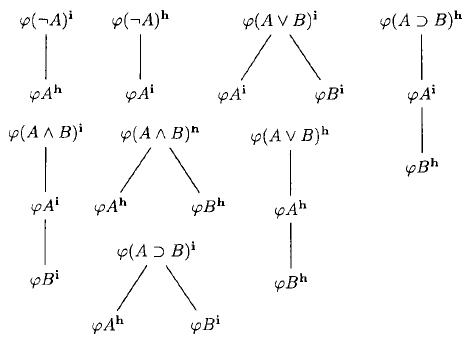
\includegraphics[width=0.7\linewidth]{img/igazsagertfa}
    \caption{Igazságértékelés-fa feltétel-előírásai.}
    \label{fig:igazsagertfa}
\end{figure}

Ezután a gyökérhez a \checkmark (feldolgozott) jelet rendeljük. Az eljárást rekurzívan folytatjuk, amíg egy ágon a fel nem dolgozott
formulák

\begin{itemize}
    \item	(a) mind ítéletváltozók nem lesznek, vagy

    \item	(b) ugyanarra a formulára egymásnak ellentmondó előírás nem jelenik meg.
\end{itemize}

Az (a) esetben az ágon előforduló ítéletváltozóknak az ágon rögzített igazságértékeit tartalmazó $n$-esek mind elemei $\varphi A^{i}$
gyökér esetén a formula igazhalmazának, $\varphi A^{h}$ gyökér esetén a formula hamishalmazának.

A (b) esetben nem áll elő ilyen igazságérték $n$-es.

\begin{figure}[H]
    \centering
    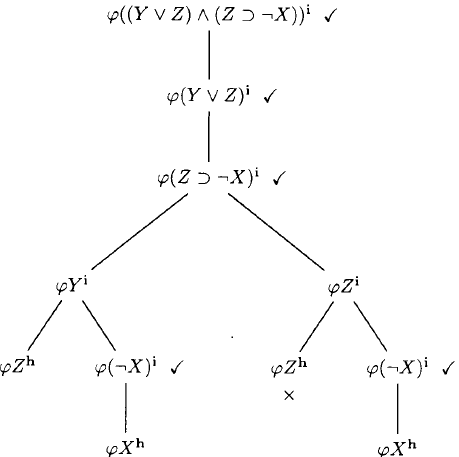
\includegraphics[width=0.5\linewidth]{img/igazsagertfapelda}
    \caption{Az $(Y \vee Z) \wedge (Z \supset \neg X)$ formula igazságértékelés-fája.}
    \label{fig:igazsagertfapelda}
\end{figure}

\noindent A fenti példában a formula igazhalmaza az igazságértékelés-fa alapján: $\left\{(i,i,h),(h,i,i),(h,i,h),(h,h,i)\right\}$\\

\noindent \textbf{Kiterjesztett igazságtábla}: Egy igazságtáblában a formula igazságértéke kiszámításának megkönnyítésére vezették
be a kiterjesztett igazságtáblát. A kiterjesztett igazságtáblában az ítéletváltozókhoz és a formulához rendelt oszlopokon kívül rendre
a formula részformuláihoz tartozó oszlopok is megjelennek. Tulajdonképpen a szerkezeti fában megjelenő részformulák vannak felsorolva.

\begin{figure}[H]
    \centering
    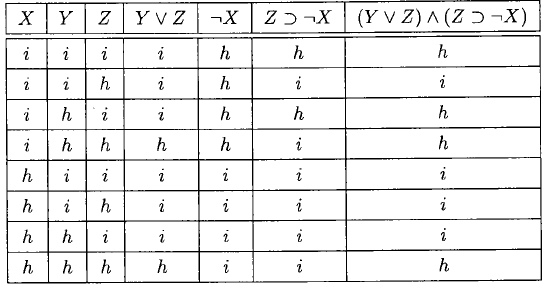
\includegraphics[width=0.5\linewidth]{img/kiterjigaztabla}
    \caption{Az $(Y \vee Z) \wedge (Z \supset \neg X)$ formula kiterjesztett igazságtáblája.}
    \label{fig:kiterjigaztabla}
\end{figure}

\noindent \textbf{Formula kielégíthetősége, modellje}: Egy $A$ ítéletlogikai formula \textit{kielégíthető}, ha létezik olyan  $\mathcal{I}$
interpretáció, melyre $\mathcal{I} \models_{0} A$, azaz a $\mathcal{B}_{\mathcal{I}}$ Boole-értékelés $A$-hoz igaz értéket rendel. Egy
ilyen interpretációt $A$ \textit{modelljének} nevezünk. Ha $A$-nak nincs modellje, akkor azt mondjuk, hogy \textit{kielégíthetetlen}.

Ha $A$ igazságtáblájában van olyan sor, amelyben a formula oszlopában igaz érték szerepel, akkor a formula kielégíthető, különben kielégíthetetlen. Ugyanígy, ha $\varphi A^{i}$ nem üres, akkor kielégíthető, különben kielégíthetetlen.\\

\noindent \textbf{Ítéletlogikai törvény, tautológia}: Egy $A$ ítéletlogikai formula \textit{ítéletlogikai törvény} vagy másképpen \textit{tautológia}, ha $\mathcal{L}_{0}$ minden interpretációja modellje $A$-nak. (jelölés: $\models_{0} A$)\\

\noindent \textbf{Eldöntésprobléma}: Eldöntésproblémának nevezzük a következő feladatokat:
\begin{enumerate}
    \item	Döntsük el tetszőleges formuláról, hogy tautológia-e!

    \item	Döntsük el tetszőleges formuláról, hogy kielégíthetetlen-e!
\end{enumerate}

\noindent \textbf{Tautologikusan ekvivalens formulák}: Az $A$ és $B$ ítéletlogikai formulák \textit{tautologikusan ekvivalensek} (jelölés: $A \sim _{0} B$), ha $\mathcal{L}_{0}$ minden $\mathcal{I}$ interpretációjában $\mathcal{B}_{\mathcal{I}}(A)=\mathcal{B}_{\mathcal{I}}(B)$.\\

\noindent \textbf{Formulahalmaz kielégíthetősége, modellje}: $\mathcal{L}_{0}$ formuláinak egy tetszőleges $\Gamma$ halmaza
kielégíthető, ha van $\mathcal{L}_{0}$-nak olyan $\mathcal{I}$ interpretációja, melyre: $\forall A \in \Gamma: \mathcal{I} \models_{0} A$.
Egy ilyen $\mathcal{I}$ interpretáció modellje $\Gamma$-nak. Ha $\Gamma$-nak nincs modellje, akkor $\Gamma$ kielégíthetetlen.\\

\noindent \textbf{Lemma}: Egy $\left\{A_{1},A_{2},...,A_{n}\right\}$ formulahalmaznak pontosan azok az $\mathcal{I}$ interpretációk
a modelljei, amelyek a $A_{1} \wedge A_{2} \wedge ... \wedge A_{n}$ formulának. Következésképpen $\left\{A_{1},A_{2},...,A_{n}\right\}$
pontosan akkor kielégíthetetlen, ha az $A_{1} \wedge A_{2} \wedge ... \wedge A_{n}$ formula kielégíthetlen.\\

\noindent \textbf{Szemantikus következmény}: Legyen $\Gamma$ ítéletlogikai formulák tetszőleges halmaza, $B$ egy tetszőleges formula.
Azt mondjuk, hogy a $B$ formula \textit{tautologikus következménye} a $\Gamma$ formulahalmaznak (jelölés: $\Gamma \models_{0} B$), ha minden olyan interpretáció, amely modellje $\Gamma$-nak, modellje $B$-nek is. A $\Gamma$-beli formulákat feltételformuláknak, vagy premisszáknak,
a B formulát következményformulának (konklúziónak) hívjuk.\\

\noindent \textbf{Tétel}: Legyen $\Gamma$ ítéletlogikai formulák tetszőleges halmaza, $A$,$B$,$C$ tetszőleges ítéletlogikai formulák.
Ha $\Gamma \models_{0} A$, $\Gamma \models_{0} B$ és $\left\{A,B\right\} \models_{0} C$, akkor $\Gamma \models_{0} C$.\\

\noindent \textbf{Tétel}: Legyenek $A_{1},A_{2},...,A_{n}, B$ tetszőleges ítéletlogikai formulák.
$\left\{A_{1},A_{2},...,A_{n}\right\} \models_{0} B$ pontosan akkor, ha a $\left\{A_{1},A_{2},...,A_{n}, \neg B\right\}$
formulahalmaz kielégíthetetlen, azaz a $A_{1} \wedge A_{2} \wedge ... \wedge A_{n} \wedge \neg B$ formula kielégíthetetlen.\\

\noindent \textbf{Tétel}: Legyenek $A_{1},A_{2},...,A_{n}, B$ tetszőleges ítéletlogikai formulák.
$\left\{A_{1},A_{2},...,A_{n}\right\} \models_{0} B$ pontosan akkor, ha
$\models_{0} A_{1} \wedge A_{2} \wedge ... \wedge A_{n} \supset B$.\\

\paragraph{Ekvivalens átalakítások}
Fogalmak:
\begin{enumerate}
    \item	Egy prímformulát (ítéletváltozót), vagy annak a negáltját közös néven \textit{literálnak} nevezünk. A prímformula
          a \textit{literál alapja}. Egy literált bizonyos esetekben \textit{egységkonjunkciónak} vagy \textit{egységdiszjunkciónak}
          (\textit{egységklóznak}) is hívunk.

    \item	\textit{Elemi konjunkció} az egységkonjunkció, illetve a különböző alapú literálok konjunkciója ($\wedge$ kapcsolat
          a literálok között). \textit{Elemi diszjunkció} vagy \textit{klóz} az egységdiszjunkció és a különböző alapú literálok
          diszjunkciója ($\vee$ kapcsolat a literálok között). Egy elemi konjunkció, illetve elemi diszjunkció \textit{teljes}
          egy $n$-változós logikai műveletre nézve, ha mind az $n$ ítéletváltozó alapja valamely literáljának.

    \item	\textit{Diszjunktív normálformának} (DNF) nevezzük az elemi konjunkciók diszjunkcióját.
          \textit{Konjunktív normálformának} (KNF) nevezzük az elemi diszjunkciók konjunkcióját. \textit{Kitüntetett}
          diszjunktív, illetve konjunktív normálformákról (KDNF, ileltve KKNF) beszélünk, ha a bennük szereplő
          elemi konjunkciók, illetve elemi diszjunkciók teljesek.

\end{enumerate}

\noindent \textbf{Tetszőleges logikai műveletet leíró KDNF, KKNF előállítása}:	Legyen $b: \mathbb{L}^{n} \to \mathbb{L}$
egy $n$-változós logikai művelet. Adjuk meg $b$ művelettábláját.
Az első $n$ oszlop fejlécébe az $X_{1}$, $X_{2}$, ... $X_{n}$ ítéletváltozókat írjuk.\\

\noindent A $b$-t leíró KDNF előállítása:

\begin{enumerate}
    \item	Válasszuk ki azokat a sorokat a művelettáblában, ahol az adott igazságérték $n$-eshez $b$ \textit{igaz}
          értéket rendel hozzá. Legyenek ezek a sorok rendre $s_{1}, s_{2}, .. s_{r}$. Minden ilyen sorhoz rendeljünk
          hozzá egy $X_{1}' \wedge X_{2}' \wedge ... \wedge X_{n}'$ teljes elemi konjunkciót úgy, hogy az $X_{j}'$ literál
          $X_{j}$ vagy $\neg X_{j}$ legyen aszerint, hogy ebben a sorban $X_{j}$ \textit{igaz} vagy \textit{hamis} igazságérték
          szerepel. Az így nyert teljes elemi konjunkciók legyenek rendre $k_{s_{1}}, k_{s_{2}}, .. k_{s_{r}}$.

    \item	Az így kapott teljes elemi konjunkciókból készítsünk egy diszjunkciós láncformulát:
          $k_{s_{1}} \vee k_{s_{2}} \vee ... \vee k_{s_{r}}$. Ez a formula lesz a $b$ művelet kitüntetett diszjunktív
          normálformája (KDNF).
\end{enumerate}

\begin{figure}[H]
    \centering
    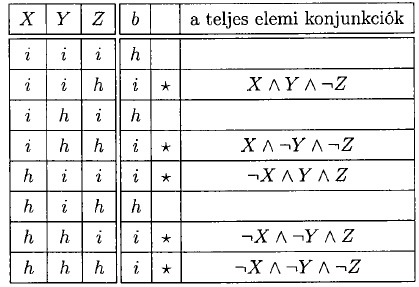
\includegraphics[width=0.5\linewidth]{img/kdnf_pelda}
    \caption{Egy háromváltozós $b$ logikai művelet művelettáblája és az előállított teljes elemi konjunkciók.}
    \label{fig:kdnf_pelda}
\end{figure}

A fenti példa $b$ műveletének kitüntetett diszjunktív normálformája a következő formula:\\
$(X \wedge Y \wedge \neg Z) \vee (X \wedge \neg Y \wedge \neg Z) \vee (\neg X \wedge Y \wedge Z) \vee (\neg X \wedge \neg Y \wedge Z) \vee (\neg X \wedge \neg Y \wedge \neg Z)$.\\

\noindent A $b$-t leíró KKNF előállítása:

\begin{enumerate}
    \item	Válasszuk ki azokat a sorokat a művelettáblában, ahol az adott igazságérték $n$-eshez $b$ \textit{hamis}
          értéket rendel hozzá. Legyenek ezek a sorok rendre $s_{1}, s_{2}, .. s_{r}$. Minden ilyen sorhoz rendeljünk
          hozzá egy $X_{1}' \vee X_{2}' \vee ... \vee X_{n}'$ teljes elemi diszjunkciót úgy, hogy az $X_{j}'$ literál
          $X_{j}$ vagy $\neg X_{j}$ legyen aszerint, hogy ebben a sorban $X_{j}$ \textit{hamis} vagy \textit{igaz} igazságérték
          szerepel. Az így nyert teljes elemi diszjunkciók legyenek rendre $d_{s_{1}}, d_{s_{2}}, .. d_{s_{r}}$.

    \item	Az így kapott teljes elemi diszjunkciókból készítsünk egy konjunkciós láncformulát:
          $d_{s_{1}} \wedge d_{s_{2}} \wedge ... \wedge d_{s_{r}}$. Ez a formula lesz a $b$ művelet kitüntetett konjunktív
          normálformája (KKNF).
\end{enumerate}

\begin{figure}[H]
    \centering
    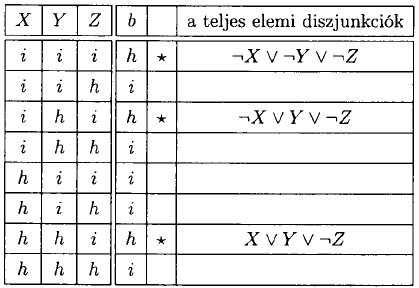
\includegraphics[width=0.5\linewidth]{img/kknf_pelda}
    \caption{Egy háromváltozós $b$ logikai művelet művelettáblája és az előállított teljes elemi diszjunkciók.}
    \label{fig:kknf_pelda}
\end{figure}

A fenti példa $b$ műveletének kitüntetett konjunktív normálformája a következő formula:\\
$(\neg X \vee \neg Y \vee \neg Z) \wedge (\neg X \vee Y \vee \neg Z) \wedge (X \vee Y \vee \neg Z)$. \\

\noindent \textbf{KNF, DNF egyszerűsítése}: Egy ítéletlogikai formula logikai összetettségén a formulában szereplő
logikai összekötőjelek számát értettük. Ugyanazt a logikai műveletet leíró formulák közül azt tekintjük egyszerűbbnek,
amelynek kisebb a logikai összetettsége (azaz kevesebb logikai összekötőjelet tartalmaz).

Legyen $X$ egy ítéletváltozó $k$ egy az $X$-et nem tartalmazó elemi konjunkció, $d$ egy $X$-et nem tartalmazó elemi
diszjunkció. Ekkor az

\begin{itemize}
    \item	(a) $(X \wedge k) \vee (\neg X \wedge k) \sim_{0} k $ és

    \item	(b) $(X \vee d) \wedge (\neg X \vee d) \sim_{0} d $
\end{itemize}

egyszerűsítési szabályok alkalmazásával konjunktív és diszjunktív normálformákat írhatunk át egyszerűbb alakba.\\

\noindent Klasszikus Quine--McCluskey-féle algoritmus KDNF egyszerűsítésére:

\begin{enumerate}
    \item	Soroljuk fel a KDNF-ben szereplő összes teljes elemi konjunkciót az $L_{0}$ listában, $j:=0$.

    \item	Megvizsgáljuk az $L_{j}$-ben szereplő összes lehetséges elemi konjunkciópárt, hogy alkalmazható-e
          rájuk az (a) egyszerűsítési szabály. Ha igen, akkor a két kiválasztott konjunkciót $\checkmark$-val megjelöljük,
          és az eredmény konjunkciót beírjuk a $L_{j+1}$ listába. Azok az elemi konjunkciók, amelyek az $L_{j}$ vizsgálata
          során nem lesznek megjelölve, nem voltak egyszerűsíthetők, tehát bekerülnek az egyszerűsített diszjunktív
          normálformába.

    \item	Ha az $L_{j+1}$ konjunkciólista nem üres, akkor $j:=j+1$. Hajtsuk végre újból a 2. lépést.

    \item	Az algoritmus során kapott, de meg nem jelölt elemi konjunkciókból készítsünk egy diszjunkciós
          láncformulát. Így az eredeti KDNF-el logikailag ekvivalens, egyszerűsített DNF-et kapunk.
\end{enumerate}

\paragraph{Rezolúció}

Legyenek $A_{1}, A_{2}, ... , A_{n}, B$ tetszőleges ítéletlogikai formulák.
Azt szeretnénk bebizonyítani, hogy $\left\{A_{1}, A_{2}, ... , A_{n}\right\} \models_{0} B$,
ami ekvivalens azzal, hogy $\left\{A_{1}, A_{2}, ... , A_{n}, \neg B\right\}$ kielégíthetetlen.
Írjuk át ez utóbbi formulahalmaz formuláit KNF alakba! Ekkor a
$\left\{KNF_{A_{1}}, KNF_{A_{2}}, ... , KNF_{A_{n}}, KNF_{\neg B}\right\}$ formulahalmazt
kapjuk, ami pontosan akkor kielégíthetetlen, ha a halmaz formuláiban szereplő klózok halmaza
kielégíthetetlen.

A klózokra vonatkozó egyszerűsítési szabály szerint ha $X$ ítéletváltozó, $C$ pedig $X$-et nem
tartalmazó klóz, akkor $(X \vee C) \wedge (\neg X \vee C) \sim_{0} C$. Az $X$ és a $\neg X$
egységklózok (azt mondjuk, hogy $X$ és $\neg X$ komplemens literálpár) konjunkciójával ekvivalens
egyszerűbb, egyetlen literált sem tartalmazó klóz az üres klóz, melyet a $\square$ jellel
jelölünk és definíció szerint minden interpretációban hamis igazságértékű.

Legyenek most $C_{1}$ és $C_{2}$ olyan klózok, melyek pontosan egy komplemens literálpárt tartalmaznak,
azaz $C_{1} = C_{1}' \vee L_{1}$ és $C_{2} = C_{2}' \vee L_{2}$, ahol $L_{1}$ és $L_{2}$ az egyetlen
komplemens literálpár ($C_{1}'$ és $C_{2}'$ üres klózok is lehetnek). Világos, hogy ha a két klózban
a komplemens literálpáron kívül is vannak literálok, és ezek nem mind azonosak, az egyszerűsítési
szabály alkalmazhatósági feltétele nem áll fenn.\\

\noindent \textbf{Tétel}: Ha $C_{1} = C_{1}' \vee L_{1}$ és $C_{2} = C_{2}' \vee L_{2}$,
ahol $L_{1}$ és $L_{2}$	komplemens literálpár, akkor $\left\{C_{1},C_{2}\right\} \models_{0} C_{1}' \vee C_{2}'$\\

\noindent \textbf{Rezolvens}: Legyenek $C_{1}$ és $C_{2}$ olyan klózok, melyek pontosan egy komplemens literálpárt tartalmaznak,
azaz $C_{1} = C_{1}' \vee L_{1}$ és $C_{2} = C_{2}' \vee L_{2}$, ahol $L_{1}$ és $L_{2}$ a komplemens literálpár,
a $C_{1}' \vee C_{2}'$ klózt a $(C_{1},C_{2})$ klózpár (vagy a $C_{1} \vee C_{2}$ formula) \textit{rezolvensének} nevezzük.
Ha $C_{1} = L_{1}$ és $C_{2} = L_{2}$ (azaz $C_{1}'$ és $C_{2}'$ üres klózok), rezolvensük az üres klóz ($\square$).
Az a tevékenység, melynek eredménye a rezolvens, a \textit{rezolválás}.

\begin{figure}[H]
    \centering
    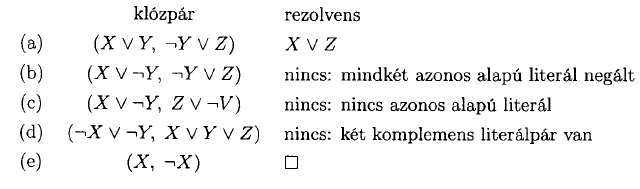
\includegraphics[width=0.7\linewidth]{img/rezolvens}
    \caption{Példák klózpárok rezolválhatóságára, rezolvensére.}
    \label{fig:rezolvens}
\end{figure}

\noindent \textbf{Tétel}: Ha a $C$ klóz a $(C_{1},C_{2})$ klózpár rezolvense, akkor azon $\mathcal{I}$ interpretációk
a $\left\{C_{1}, C_{2}\right\}$ klózhalmazt nem elégíthetik ki, amelyekben $C$ igazságértéke hamis, azaz
$\mathcal{B}_{\mathcal{I}}(C) = hamis$.\\

\noindent \textbf{Rezolúciós levezetés}: Egy $S$ klózhalmazból a $C$ klóz rezolúciós levezetése egy olyan véges
$k_{1}, k_{2}, ... ,k_{m} (m \geq 1)$ klózsorozat, ahol minden $j = 1, 2, ..., m$-re

\begin{enumerate}
    \item	vagy $k_{j} \in S$,

    \item	vagy van olyan $1 \leq s,t \le j$, hogy $k_{j}$ a $(k_{s}, k_{t})$ klózpár rezolvense,
\end{enumerate}

\noindent és a klózsorozat utolsó tagja, $k_{m}$, éppen a $C$ klóz.

Megállapodásunk szerint a rezolúciós kalkulus eldöntésproblémája az, hogy levezethető-e $S$-ből $\square$. A
rezolúciós levezetés célja tehát $\square$ levezetése $S$-ből. Azt, hogy $\square$ levezethető $S$-ből,
úgy is ki lehet fejezni, hogy létezik $S$-nek rezolúciós cáfolata.\\

\noindent Példa: Próbáljuk meg levezetni $\square$-t az
$S = \left\{\neg X \vee Y, \neg Y \vee Z, X \vee Z, \neg V \vee Y \vee Z, \neg Z \right\}$
klózhalmazból. A levezetés bármelyik $S$-beli klózból indítható.

\begin{figure}[H]
    \centering
    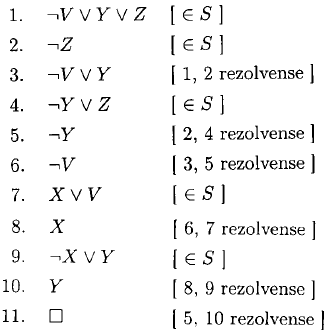
\includegraphics[width=0.4\linewidth]{img/rezoluciopelda}
    \caption{$\square$ rezolúciós levezetése $S$-ből.}
    \label{fig:rezoluciopelda}
\end{figure}

\noindent \textbf{Lemma}: Legyen $S$ tetszőleges klózhalmaz. $S$-ből történő rezolúciós levezetés esetén bármely $S$-ből
levezetett klóz tautologikus következménye $S$-nek.\\

\noindent \textbf{A rezolúciós kalkulus helyessége}: A rezolúciós kalkulus \textit{helyes}, azaz tetszőleges
$S$ klózhalmaz esetén amennyiben $S$-ből levezethető $\square$, akkor $S$ \textit{kielégíthetetlen}.\\

\noindent \textbf{A rezolúciós kalkulus teljessége}: A rezolúciós kalkulus \textit{teljes}, azaz bármely véges, kielégíthetetlen
$S$ klózhalmaz esetén $S$-ből levezethető $\square$.\\

\noindent \textbf{Levezetési fa}: Egy rezolúciós levezetés szerkezetét \textit{levezetési fa} segítségével szemléltethetjük.
A levezetési fa csúcsai klózok. Két csúcsból pontosan akkor vezet él egy harmadik, közös csúcsba, ha az a két klóz rezolvense.

\begin{figure}[H]
    \centering
    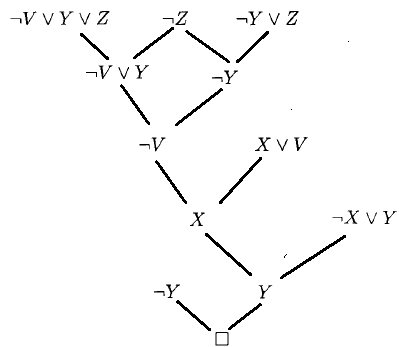
\includegraphics[width=0.5\linewidth]{img/rezoluciopelda_levfa}
    \caption{Az előző példa levezetési fája.}
    \label{fig:rezoluciopelda_levfa}
\end{figure}

\noindent \textbf{Rezolúciós stratégiák}:

\begin{itemize}
    \item	\textit{Lineáris rezolúció}: Egy $S$ klózhalmazból való lineáris rezolúciós levezetés egy olyan
          $k_{1},l_{1},k_{2},l_{2}, ..., k_{m-1},l_{m-1}, k_{m}$ rezolúciós levezetés, amelyben minden
          $j = 2, 3, ..., m$-re $k_{j}$ a $(k_{j-1},l_{j-1})$ klózpár rezolvense. A $k_{j}$ klózokat centrális
          klózoknak, az $l_{j}$ klózokat mellékklózoknak nevezzük.

          Tetszőleges rezolúciós levezetés átírható lineárissá, azaz a lineáris rezolúciós kalkulus teljes.

    \item	\textit{Lineáris inputrezolúció}: Egy $S$ klózhalmazból való lineáris inputrezolúciós levezetés
          egy olyan $k_{1},l_{1},k_{2},l_{2}, ..., k_{m-1},l_{m-1}, k_{m}$ lineáris rezolúciós levezetés, amelyben minden
          $j = 1, 2, ..., m-1$-re $l_{j} \in S$, azaz a lineáris inputrezolúciós levezetésben a mellékklózok $S$ elemei.

          A lineáris inputrezolúciós stratégia nem teljes, de megadható olyan formulaosztály, melyre az. A legfeljebb egy
          negált literált tartalmazó klózokat Horn-klózoknak nevezzük, a Horn-formulák pedig azok a formulák, melyek
          konjunktív normálformája Horn-klózok konjunkciója. A lineáris inputrezolúciós stratégia Horn-formulák esetén teljes.
\end{itemize}

\subsection{Predikátumkalkulus}

\subsubsection{Elsőrendű logikai nyelvek szintaxisa}

Egy elsőrendű logikai nyelv ábécéje logikai és logikán kívüli szimbólumokat, továbbá elválasztójeleket tartalmaz.
A logikán kívüli szimbólumhalmaz megadható $<Srt, Pr, Fn, Cnst>$ alakban, ahol:

\begin{enumerate}
    \item	$Srt$ nemüres halmaz, elemei fajtákat szimbolizálnak,

    \item	$Pr$ nemüres halmaz, elemei predikátumszimbólumok,

    \item	az $Fn$ halmaz elemei függvényszimbólumok,

    \item	$Cnst$ pedig a függvényszimbólumok halmaza.
\end{enumerate}

\noindent Az $<Srt, Pr, Fn, Cnst>$ ábécé szignatúrája egy $<\nu_{1}, \nu_{2}, \nu_{3}>$ hármas, ahol

\begin{enumerate}
    \item	minden $P \in Pr$ predikátumszimbólumhoz $\nu_{1}$ a predikátumszimbólum alakját,
          azaz a $(\pi_{1}, \pi_{2}, ..., \pi_{k})$ fajtasorozatot,

    \item	minden $f \in Fn$ függvényszimbólumhoz $\nu_{2}$ a függvényszimbólum alakját,
          azaz a $(\pi_{1}, \pi_{2}, ..., \pi_{k}, \pi)$ fajtasorozatot és

    \item	minden $c \in Cnst$ konstansszimbólumhoz $\nu_{3}$ a konstansszimbólumhoz alakját,
          azaz $(\pi)$-t
\end{enumerate}

\noindent rendel ($k > 0$ és $\pi_{1}, \pi_{2}, ..., \pi_{k}, \pi \in Srt$).

Logikai jelek az ítéletlogikában is használt logikai összekötőjelek, valamint az univerzális ($\forall$)
és egzisztenciális ($\exists$) kvantorok és a különböző fajtájú individuumváltozók. Egy elsőrendű
nyelv ábécéjében minden $\pi \in Srt$ fajtához szimbólumoknak megszámlálhatóan végtelen
$v_{1}^{\pi}, v_{2}^{\pi}, ...$ rendszere tartozik, ezeket a szimbólumokat nevezzük $\pi$ fajtájú
változóknak. Elválasztójel a nyitó és csukó zárójelek, és a vessző.

Az elsőrendű logikai nyelvekben az elválasztójelek és a logikai jelek mindig ugyanazok, viszont
a logikán kívüli jelek halmaza, illetve ezek szignatúrája nyelvről nyelvre lényegesen különbözhet.
Ezért mindig megadjuk a $<Srt, Pr, Fn, Cnst>$ négyest és ennek $<\nu_{1}, \nu_{2}, \nu_{3}>$
szignatúráját, amikor egy elsőrendű logikai nyelv ábécéjére hivatkozunk. Jelölése $V[V_{\nu}]$,
ahol $V_{\nu}$ adja meg a $<\nu_{1}, \nu_{2}, \nu_{3}>$ szignatúrájú $<Srt, Pr, Fn, Cnst>$ négyest.\\

\noindent \textbf{Termek}: A $V[V_{\nu}]$ ábécé feletti termek halmaza $\mathcal{L}_{t}[V_{\nu}]$, ami
a következő tulajdonságokkal bír:

\begin{enumerate}
    \item	Minden $\pi \in Srt$ fajtájú változó és konstans $\pi$ fajtájú term.

    \item	Ha az $f \in Fn$ függvényszimbólum $(\pi_{1}, \pi_{2}, ..., \pi_{k}, \pi)$ alakú
          és $t_{1}, t_{2}, ..., t_{k}$ -- rendre $\pi_{1}, \pi_{2}, ..., \pi_{k}$ fajtájú -- termek,
          akkor az $f(s_{1}, s_{2}, ..., s_{k})$ egy $\pi$ fajtájú term.

    \item	Minden term az 1-2. szabályok véges sokszori alkalmazásával áll elő.
\end{enumerate}

\noindent \textbf{Formulák}: A $V[V_{\nu}]$ ábécé feletti elsőrendű formulák halmaza $\mathcal{L}_{f}[V_{\nu}]$, ami
a következő tulajdonságokkal bír:

\begin{enumerate}
    \item	Ha a $P \in Pr$ predikátumszimbólum $(\pi_{1}, \pi_{2}, ..., \pi_{k})$ alakú
          és az $t_{1}, t_{2}, ..., t_{k}$ -- rendre $\pi_{1}, \pi_{2}, ..., \pi_{k}$ fajtájú --
          termek, akkor a $P(t_{1}, t_{2}, ..., t_{k})$ szó egy elsőrendű formula.
          Az így nyert formulákat atomi formuláknak nevezzük.

    \item	Ha $S$ elsőrendű formula, akkor $\neg S$ is az.

    \item	Ha $S$ és $T$ elsőrendű formulák és $\circ$ binér logikai összekötőjel,
          akkor $(S \circ T)$ is elsőrendű formula.

    \item	Ha $S$ eleme elsőrendű formula, $Q$ kvantor ($\forall$ vagy $\exists$) és $x$
          tetszőleges változó, akkor $QxS$ is elsőrendű formula. Az így nyert formulákat kvantált formuláknak nevezzük,
          a $\forall xS$ alakú formulák univerzálisan kvantált formulák, a $\exists xS$ alakú formulák
          pedig egzisztenciálisan kvantált formulák. A kvantált formulákban $Qx$ a formula prefixe, $S$
          pedig a magja.

    \item	Minden elsőrendű formula az 1-4. szabályok véges sokszori alkalmazásával áll elő.
\end{enumerate}

\noindent A $V[V_{\nu}]$ ábécé feletti elsőrendű logikai nyelv
$\mathcal{L}[V_{\nu}] = \mathcal{L}_{t}[V_{\nu}] \cup \mathcal{L}_{f}[V_{\nu}]$, azaz $\mathcal{L}[V_{\nu}]$
minden szava vagy term, vagy formula.\\

A negációs, konjunkciós, diszjunkciós, implikációs (ezek jelentése ua., mint nulladrendben) és kvantált formulák
összetett formulák.

Az elsőrendű logikai nyelv prímformulái az atomi formulák és a kvantált formulák.\\

\noindent \textbf{Változóelőfordulás fajtái}: Egy formula $x$ változójának egy előfordulása:

\begin{itemize}
    \item	szabad, ha nem esik $x$-re vonatkozó kvantor hatáskörébe,

    \item	kötött, ha $x$-re vonatkozó kvantor hatáskörébe esik.
\end{itemize}

\noindent \textbf{Változó fajtái}: Egy formula $x$ változója:

\begin{itemize}
    \item	szabad, ha minden előfordulása szabad,

    \item	kötött, ha minden előfordulása kötött, és

    \item	vegyes, ha van szabad és kötött előfordulása is.
\end{itemize}

\noindent \textbf{Formula zártsága, nyíltsága}: Egy formula:

\begin{itemize}
    \item	zárt, ha minden változója kötött,

    \item	nyílt, ha legalább egy változójának van szabad előfordulása és

    \item	kvantormentes, ha nincs benne kvantor
\end{itemize}

Megjegyzés: a zárt formulák elsőrendű állításokat szimbolizálnak (egy elsőrendű állítás nem más, mint elemek egy halmazára
megfogalmazott kijelentő mondat).

\subsubsection{Az elsőrendű logika szemantikája}

\noindent \textbf{Matematikai struktúra}: Matematikai struktúrán egy $<U, R, M, K>$ négyest értünk, ahol:

\begin{enumerate}
    \item	$U = \bigcup_{\pi} U_{\pi}$ nem üres alaphalmaz (univerzum),

    \item	$R$ az $U$-n értelmezett logikai függvények (relációk) halmaza,

    \item	$M$ az $U$-n értelmezett matematikai függvények (alapműveletek) halmaza,

    \item	$K$ az $U$ kijelölt elemeinek (konstansainak) halmaza (lehet üres).
\end{enumerate}

\noindent \textbf{Interpretáció}: Az interpretáció egy $<U, R, M, K>$ matematikai struktúra és
$\mathcal{I} = <\mathcal{I}_{Srt}, \mathcal{I}_{Pr}, \mathcal{I}_{Fn}, \mathcal{I}_{Cnst}>$
függvénynégyes, ahol:

\begin{itemize}
    \item	az $\mathcal{I}_{Srt} : \pi \mapsto U_{\pi}$ függvény megad minden egyes $\pi \in Srt$ fajtához
          egy $U_{\pi}$ nemüres halmazt, a $\pi$ fajtájú individuumok halmazát,

    \item	az $\mathcal{I}_{Pr} : P \mapsto P^{\mathcal{I}}$ függvény megad minden
          $(\pi_{1}, \pi_{2}, ..., \pi_{k})$ alakú $P \in Pr$ predikátumszimbólumhoz egy
          $P^{\mathcal{I}} : U_{\pi_{1}} \times U_{\pi_{2}} \times ... \times U_{\pi_{k}} \to \mathbb{L}$
          logikai függvényt (relációt),

    \item	az $\mathcal{I}_{Fn} : f \mapsto f^{\mathcal{I}}$ függvény hozzárendel minden
          $(\pi_{1}, \pi_{2}, ..., \pi_{k}, \pi)$ alakú $f \in Fn$ függvényszimbólumhoz egy
          $P^{\mathcal{I}} : U_{\pi_{1}} \times U_{\pi_{2}} \times ... \times U_{\pi_{k}} \to U_{\pi}$
          matematikai függvényt (műveletet),

    \item	az $\mathcal{I}_{Cnst} : c \mapsto ct^{\mathcal{I}}$ pedig minden $\pi$ fajtájú
          $c \in Cnst$ konstansszimbólumhoz az $U_{\pi}$ individuumtartománynak egy individuumát
          rendeli, azaz $c^{\mathcal{I}} \in U_{\pi}$.
\end{itemize}

\noindent \textbf{Változókiértékelés}: Legyen az $\mathcal{L}[V_{\nu}]$ nyelvnek $\mathcal{I}$ egy interpretációja,
az interpretáció univerzuma legyen U és jelölje V a nyelv változóinak halmazát. Egy olyan $\kappa : V \to U$ leképezést,
ahol ha $x$ $\pi$ fajtájú változó, akkor $\kappa(x) \in U_{\pi}$, $\mathcal{I}$-beli változókiértékelésnek nevezünk.\\

\noindent \textbf{$\mathcal{L}_{t}[V_{\nu}]$ szemantikája}:
Legyen az $\mathcal{L}[V_{\nu}]$ nyelvnek $\mathcal{I}$ egy interpretációja és $\kappa$ egy $\mathcal{I}$-beli
változókiértékelés. Az $\mathcal{L}[V_{\nu}]$ nyelv egy $\pi$ fajtájú $t$ termjének értéke $\mathcal{I}$-ben
a $\kappa$ változókiértékelés mellett az alábbi -- $|t|^{\mathcal{I},\kappa}$-val jelölt -- $U_{\pi}$-beli
individuum:

\begin{enumerate}
    \item	ha $c \in Cnst$ $\pi$ fajtájú konstansszimbólum, akkor $|c|^{\mathcal{I},\kappa}$ az $U_{\pi}$-beli
          $c^{\mathcal{I}}$ individuum,

    \item	ha $x$ $\pi$ fajtájú változó, akkor $|x|^{\mathcal{I},\kappa}$ az $U_{\pi}$-beli $\kappa(x)$ individuum,

    \item	ha $t_{1}, t_{2}, ..., t_{k}$ rendre $\pi_{1}, \pi_{2}, ..., \pi_{k}$ fajtájú termek és ezek értékei
          a $\kappa$ változókiértékelés mellett rendre az $U_{\pi_{1}}$-beli $|t_{1}|^{\mathcal{I},\kappa}$, az
          $U_{\pi_{2}}$-beli $|t_{2}|^{\mathcal{I},\kappa}$ ... és az $U_{\pi_{k}}$-beli $|t_{k}|^{\mathcal{I},\kappa}$
          individuumok, akkor egy $(\pi_{1}, \pi_{2}, ..., \pi_{k}, \pi)$ alakú $f \in Fn$ függvényszimbólum esetén
          $|f(t_{1}, t_{2}, ..., t_{k})|^{\mathcal{I},\kappa}$ az $U_{\pi}$-beli
          $f^{\mathcal{I}}(|t_{1}|^{\mathcal{I},\kappa}, |t_{2}|^{\mathcal{I},\kappa}, ..., |t_{k}|^{\mathcal{I},\kappa})$
          individuum.

\end{enumerate}

\noindent \textbf{Változókiértékelés $x$-variánsa}: Legyen $x$ egy változó. A $\kappa^{*}$ változókiértékelés a
$\kappa$ változókiértékelés $x$-variánsa, ha $\kappa^{*}(y) = y$ minden $x$-től különböző $y$ változó esetén.\\

\noindent \textbf{Elsőrendű logikai formula logikai értéke}:
Legyen az $\mathcal{L}[V_{\nu}]$ nyelvnek $\mathcal{I}$ egy interpretációja és $\kappa$ egy $\mathcal{I}$-beli
változókiértékelés. Az $\mathcal{L}[V_{\nu}]$ nyelv egy $C$ formulájához $\mathcal{I}$-ben a $\kappa$ változókiértékelés
mellett az alábbi -- $|C|^{\mathcal{I},\kappa}$-val jelölt -- igazságértéket rendeljük:

\begin{enumerate}
    \item	$|P(t_{1}, t_{2}, ..., t_{k})|^{\mathcal{I},\kappa} = \left\{
              \begin{array}{lr}
                  igaz  & : P^{\mathcal{I}}(|t_{1}|^{\mathcal{I},\kappa}, |t_{2}|^{\mathcal{I},\kappa}, ..., |t_{k}|^{\mathcal{I},\kappa}) = igaz \\
                  hamis & : kulonben
              \end{array}
              \right\}$

    \item	$|\neg A|^{\mathcal{I},\kappa}$ legyen $\neg |A|^{\mathcal{I},\kappa}$

    \item	$|A \wedge B|^{\mathcal{I},\kappa}$ legyen $|A|^{\mathcal{I},\kappa} \wedge |B|^{\mathcal{I},\kappa}$

    \item	$|A \vee B|^{\mathcal{I},\kappa}$ legyen $|A|^{\mathcal{I},\kappa} \vee |B|^{\mathcal{I},\kappa}$

    \item	$|A \supset B|^{\mathcal{I},\kappa}$ legyen $|A|^{\mathcal{I},\kappa} \supset |B|^{\mathcal{I},\kappa}$

    \item	$|\forall x A|^{\mathcal{I},\kappa} = \left\{
              \begin{array}{lr}
                  igaz  & : |A|^{\mathcal{I},\kappa^{*}} = igaz \ \kappa \ minden \ \kappa^{*} \ x-variansara \\
                  hamis & : kulonben
              \end{array}
              \right\}$

    \item	$|\exists x A|^{\mathcal{I},\kappa} = \left\{
              \begin{array}{lr}
                  igaz  & : |A|^{\mathcal{I},\kappa^{*}} = igaz \ \kappa \ valamely \ \kappa^{*} \ x-variansara \\
                  hamis & : kulonben
              \end{array}
              \right\}$

\end{enumerate}

\noindent \textbf{Elsőrendű formula kielégíthetősége}: Egy $A$ elsőrendű formula kielégíthető, ha van
olyan $\mathcal{I}$ interpretáció és $\kappa$ változókiértékelés, amelyre $|A|^{\mathcal{I},\kappa} = igaz$
(ekkor azt mondjuk, hogy az $\mathcal{I}$ interpretáció és $\kappa$ változókiértékelés kielégíti $A$-t),
különben kielégíthetetlen.

Amennyiben az $A$ formula zárt, igazságértékét egyedül az interpretáció határozza meg. Ha $|A|^{\mathcal{I}} = igaz$,
azt mondjuk, hogy az $\mathcal{I}$ kielégíti $A$-t vagy másképpen: $\mathcal{I}$ modellje $A$-nak ($\mathcal{I} \models A$).\\

\noindent \textbf{Logikailag igaz elsőrendű formula}: Egy $A$ elsőrendű logikai formula logikailag igaz,
ha minden $\mathcal{I}$ interpretációban és $\mathcal{I}$ minden $\kappa$ változókiértékelése mellett
$|A|^{\mathcal{I},\kappa} = igaz$. Jelölése: $\models A$.\\

\noindent \textbf{Szemantikus következmény}: Azt mondjuk, hogy a $G$ formula \textit{szemantikus következménye} az
$\mathcal{F}$ formulahalmaznak, ha minden olyan $\mathcal{I}$ interpretációra, amelyre $\mathcal{I} \models \mathcal{F}$
fennáll, $\mathcal{I} \models G$ is igaz (jelölés: $\mathcal{F} \models G$).\\

\noindent \textbf{Tétel}: Legyenek $A_{1}, A_{2}, ..., A_{n}, B$ ($n \geq 1$) tetszőleges, ugyanabból az elsőrendű logikai nyelvből
való formulák. Ekkor $\left\{A_{1}, A_{2}, ..., A_{n}\right\} \models B$ akkor és csak akkor, ha
$A_{1} \wedge A_{2} \wedge ... \wedge A_{n} \wedge \neg B$ kielégíthetetlen.\\

\noindent \textbf{Rezolúció}: Elsőrendű predikátumkalkulusban is végezhető rezolúció, ráadásul a módszer
helyes és teljes is. Nehézséget a klózok kialakítása okozhat, amelyek zárt,
univerzálisan kvantált literálok konjunkciójából állnak. Ehhez eszközeink a
prenex-, illetve skolem-formák.

\end{document}